\documentclass[10pt,a4paper]{article}
\usepackage[utf8]{inputenc}
\usepackage[german]{babel}
\usepackage[T1]{fontenc}
\usepackage{amsmath}
\usepackage{amsfonts}
\usepackage{amssymb}
\usepackage{graphicx}
\title{Wechselströme}
\begin{document}
\section*{Wechselströme(AC)}
\begin{itemize}
\item ändert Richtung (Polung) periodisch.
\item Strom ist im zeitlichen Mittel null.
\item $U(t)=U_0 sin(\omega t)$
\end{itemize}
\subsection{Impedanz(Wechselstromwiderstände)}
\begin{itemize}
\item Kondensatoren und Spulen verhalten sich bei Wechselstrom ähnlich wie Widerstände, verschieben aber zusätzlich den Phasenwinkel zwischen Strom und Spannungsverlauf.
\item[Ohmscher Widerstand:] $Z_R=R \Rightarrow$ keine Phasenverschiebung
\item[Kondensator:] $Z_C=\frac{1}{i\omega C} \Rightarrow$ Spannung um 90 grad verzögert.
\item[Spule:] $Z_L=i\omega L \Rightarrow$ Spannung eilt Strom um 90 Grad voraus.
\end{itemize}
\fbox{Bei Induktivitäten die Ströme sich verspäten.}
\subsection{Leistung}
\begin{equation}
P(t)=U(t)\cdot I(t)
\end{equation}
\subsubsection{Wirkleistung(P)}
Leistung, die für die Umwandlung in andere Leistungen (thermisch, mechanisch, chemisch) verfügbar ist. 
\begin{itemize}
\item[bei Gleichströmen] $P_{Wirk}=P=UI $
\item[bei Wechselstrom]
\begin{align}
P_{Wirk}&=\bar{P}=\bar{U}\bar{I} \hspace{1,0cm} (\bar{P}=\text{Augenblicklistung)} \notag \\
&= \frac{1}{T}=\int^{t_0}_{t_0+T}{U\cdot I dt} \notag \\
&\Rightarrow P_{Wirk}=U \cdot I \cdot cos(\phi) 
\end{align} 
\end{itemize}
\subsubsection{Blindleistung}
Zusätzliche Energie, die nicht zur Wirkleistung beiträgt. Es fließt bei der Übertragung mehr Energie als der Verbraucher in derselben Anzahl von Perioden umsetzen kann. Die Blindleistung wird nicht verbraucht, also auch nicht als Stromverbrauch berechnet. Sie muss trotzdem vom Stromlieferanten bereitgestellt werden.
\begin{equation}
Q=U \cdot I \cdot sin(\phi)
\end{equation}
\subsubsection{Scheinleistung(S)}
\begin{itemize}
\item Ist bei der Leistungsaufnahme eines Geräts neben der Wirkleistung auch Blindleistung dabei, dann wird die Gesamtleistung als Scheinleistung bezeichnet.
\item Bei Gleichspannung, ist die Scheinleistung gleich der Wirkleistung P. 
\item Die Scheinleistung ist in der Regel größer als die Wirkleistung.
\end{itemize}
\begin{equation}
S=\sqrt{P^2+Q^2}
\end{equation}
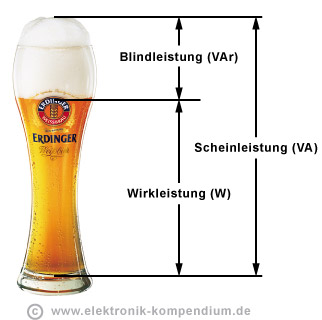
\includegraphics[scale=0.5]{beer.png}\centering 
\end{document}